% Replace the existing fig:roadmap environment AND the next two paragraphs.
% Compile from workshop_v2/论文/. Keep exactly one fig:roadmap label.
\begin{figure}[htbp]\centering
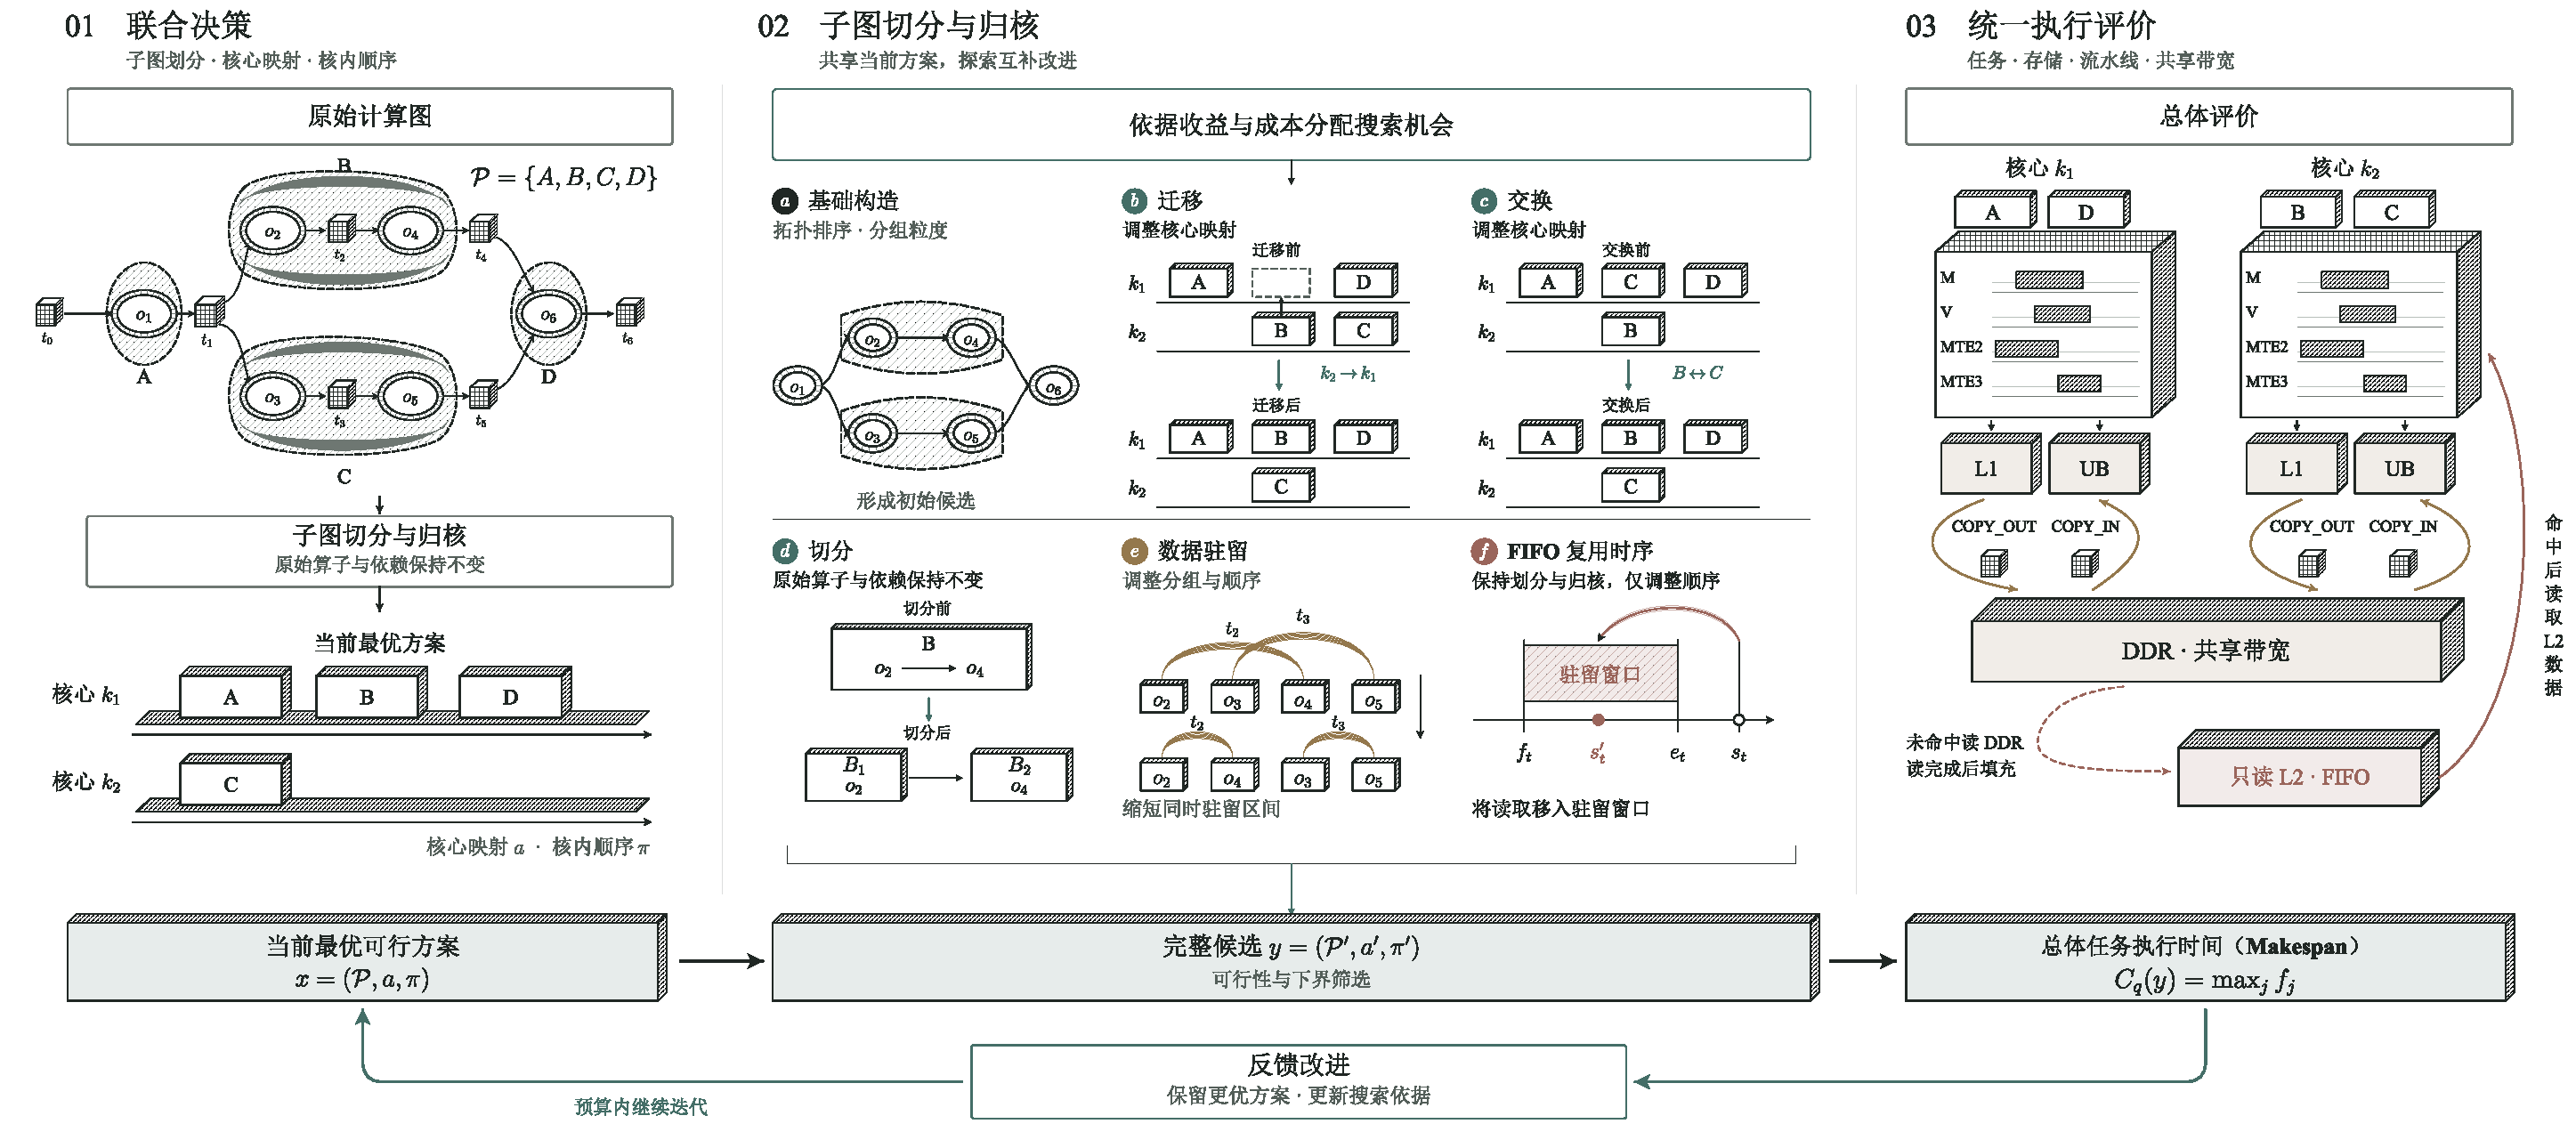
\includegraphics[width=\textwidth]{../../../../paper_a_figures/engraved_workflow/ink_v11/exports/workflow_qinglu_v11.pdf}
\caption{联合决策、子图切分与归核及统一执行评价}\label{fig:roadmap}
\end{figure}

如图~\ref{fig:roadmap} 所示，首先将子图划分、核心映射与核内顺序组成完整方案，再通过基础构造、迁移、交换、切分、数据驻留和FIFO复用时序调整生成候选，其中问题一使用（a）—（d），问题二扩展至（e），问题三扩展至（f），各操作并非串行步骤。候选经可行性与下界筛选后，在任务、存储、流水线及共享带宽约束下统一评价，按总体任务执行时间、总额外数据搬运量的优先顺序比较，保留更优可行方案，并依据收益与成本调整后续搜索机会。第三问的\texttt{COPY\_IN}在发射时查询只读L2，命中时读取其驻留数据，未命中则读取DDR；读入完成后按容量及FIFO规则尝试填充，\texttt{COPY\_OUT}仍写入DDR。上述过程循环至预算耗尽，输出当前最优可行方案，再固定第三问方案进行无L2与有L2的配对评价。
